\documentclass[20pt,margin=1in,innermargin=-4.5in,blockverticalspace=-0.25in]{tikzposter}
\geometry{paperwidth=42in,paperheight=30in}
\usepackage[utf8]{inputenc}
\usepackage{amsmath}
\usepackage{amsfonts}
\usepackage{amsthm}
\usepackage{amssymb}
\usepackage{mathrsfs}
\usepackage{graphicx}
\usepackage{caption}
\usepackage{subcaption}
\usepackage{adjustbox}
\usepackage{enumitem}
\usepackage[backend=bibtex,style=numeric,doi=false,url=false,eprint=false,sorting=none]{biblatex}
\usepackage{uofa-theme}
\usetikzlibrary{positioning,shapes,arrows}

\usepackage{mwe} % for placeholder images

\addbibresource{ref.bib}
\AtBeginBibliography{\footnotesize}

% set theme parameters
\tikzposterlatexaffectionproofoff
\usetheme{UofATheme}
\usecolorstyle{UofAStyle}

\title{GRAVI: Gene Regulatory Analysis Using Variable Inputs}
\author{\centering \textbf{Stephen M Pederson}\textsuperscript{1,2}, Geraldine Laven-Law\textsuperscript{1}, Richard Iggo\textsuperscript{1,3}, Amy Dwyer\textsuperscript{1}, Theresa E Hickey\textsuperscript{1} and Wayne D Tilley\textsuperscript{1}}
\institute{
  \textsuperscript{1}Dame Roma Mitchell Cancer Research Laboratories, Adelaide Medical School, University of Adelaide\\
  \textsuperscript{2}Black Ochre Data Laboratories, Telethon Kids Institute\\[2mm]
  \textsuperscript{3}Bordeaux Institute of Oncology, University of Bordeaux
}
%\titlegraphic{\includegraphics[width=0.1\textwidth]{UoA-standard-vert-rgb.jpg}}

% begin document
\begin{document}
\maketitle

\node [below right=15mm and 2cm] at (bottomleft |- topright) {\includegraphics[width=0.09\textwidth]{UoA-standard-vert-rgb.jpg}};
\node [below left=15mm and 2cm] at (topright) {
\includegraphics[width=0.09\textwidth]{tki.jpg}};



\centering
\begin{columns}
    \column{0.32}
    \block{Aim: Identification of Key Regulatory Targets}{
    
	    The GRAVI workflow was built to integrate ChIP-Seq, HiC, RNA-Seq and Histone marks to identify key regulatory targets.
	    The workflow was designed specifically for \textbf{multiple transcription factors to discover shared regulatory targets} in response to treatment and is available from \texttt{www.github.com/steveped/GRAVI}\\[-5mm]
	    
	    The motivating question was the joint response of the Androgen Receptor (AR) and Estrogen Receptor (ER) in response to DHT-treatment, across multiple cell lines combined with changes to the histone mark H3K27ac.
	    This research currently offers an exciting new therapeutic approach to ER$^+$ breast cancer\cite{Hickey2021}.

    }
    \block{GRAVI Outline}{
	    The GRAVI workflow is written in \texttt{snakemake} and produces a set of linked \texttt{html} pages with all code visible and all results presented clearly in a manner inspired by the \texttt{workflowr} package\cite{workflowr}.
	    This makes for completely reproducible results which are comparable across multiple datasets (e.g. multiple cell lines or tissues), and are easily accessible for collaborators.
	    The minimal input is one ChIP-Seq target across two conditions with the following steps always performed:\\[-8mm]
    
    	\begin{enumerate}[itemsep=0mm]
    		\item Prepare Annotations
    		\item Identify Consensus Peaks
    		\item Identify Differentially Bound Regions
    	\end{enumerate}

        \begin{tikzfigure}[\textbf{GRAVI Outline} ChIP-Seq inputs are shown in green]
        	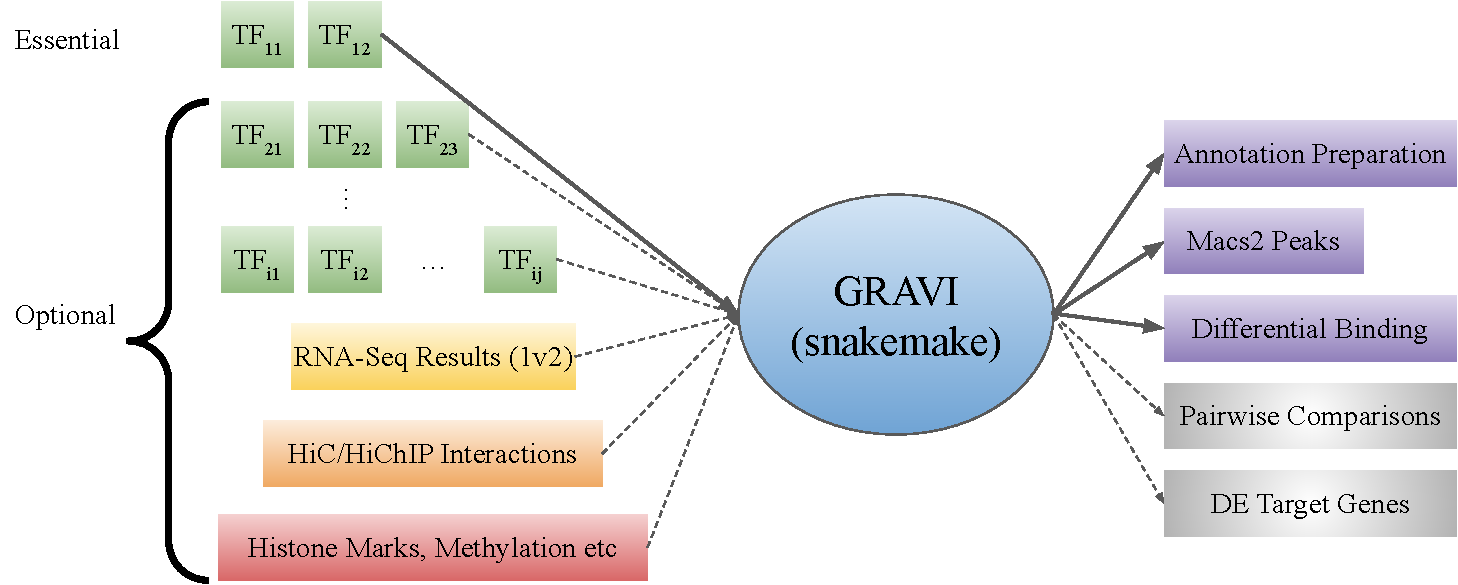
\includegraphics[width=0.78\linewidth]{GRAVI_Diagram-crop}
        \end{tikzfigure}
    	
    	Incorporation of multiple ChIP targets will enable \textbf{pairwise comparisons} to be performed on differential binding results to find shared responsive regulatory regions.
    	Likewise the addition of results from RNA-Seq analyses will provide direct evidence of changed gene expression from treatment responsive regulatory regions.
    	Pathway enrichment is performed within each step of the analysis, with the workflow being heavily dependent on the \texttt{extraChIPs} Bioconductor package\cite{extraChIPs}.
    

    }
    \block{Annotation Preparation}{
    A set of \textit{non-overlapping genomic regions} is defined for the specific annotations utilised, and incorporating all \textbf{transcript-level} information with genomic distances defined by the user.
    Regions are defined as 1) Promoter, 2) Upstream Promoter, 3)Exon, 4) Intron, 5) Proximal Intergenic, and 6) Distal Intergenic.
    The relationship between defined regions and any provided genomic features (e.g. H3K27ac) data or any long-range interactions (e.g. HiC) is also assessed.
    Standardised colour schemes are also defined for propagation through the workflow.
    }

    \column{0.36}
    \block{Peak Calling}{
    	
    	Macs2 callpeak\cite{macs2} is used for identifying peaks within individual replicates and across all replicates within a treatment group.
    	QC on each sample is performed identifying using common metrics such as FRIP with the relationship between all samples assessed using UpSet Plots and VennDiagrams.
    	Consensus peaks are identified with treatment groups and across all samples with all regions exported as \texttt{bed} files.\\[-5mm]
    	
        \begin{tikzfigure}[Example outputs for ER binding showing all samples as an UpSet plots, common consensus peaks  and the genomic distribution.]
        	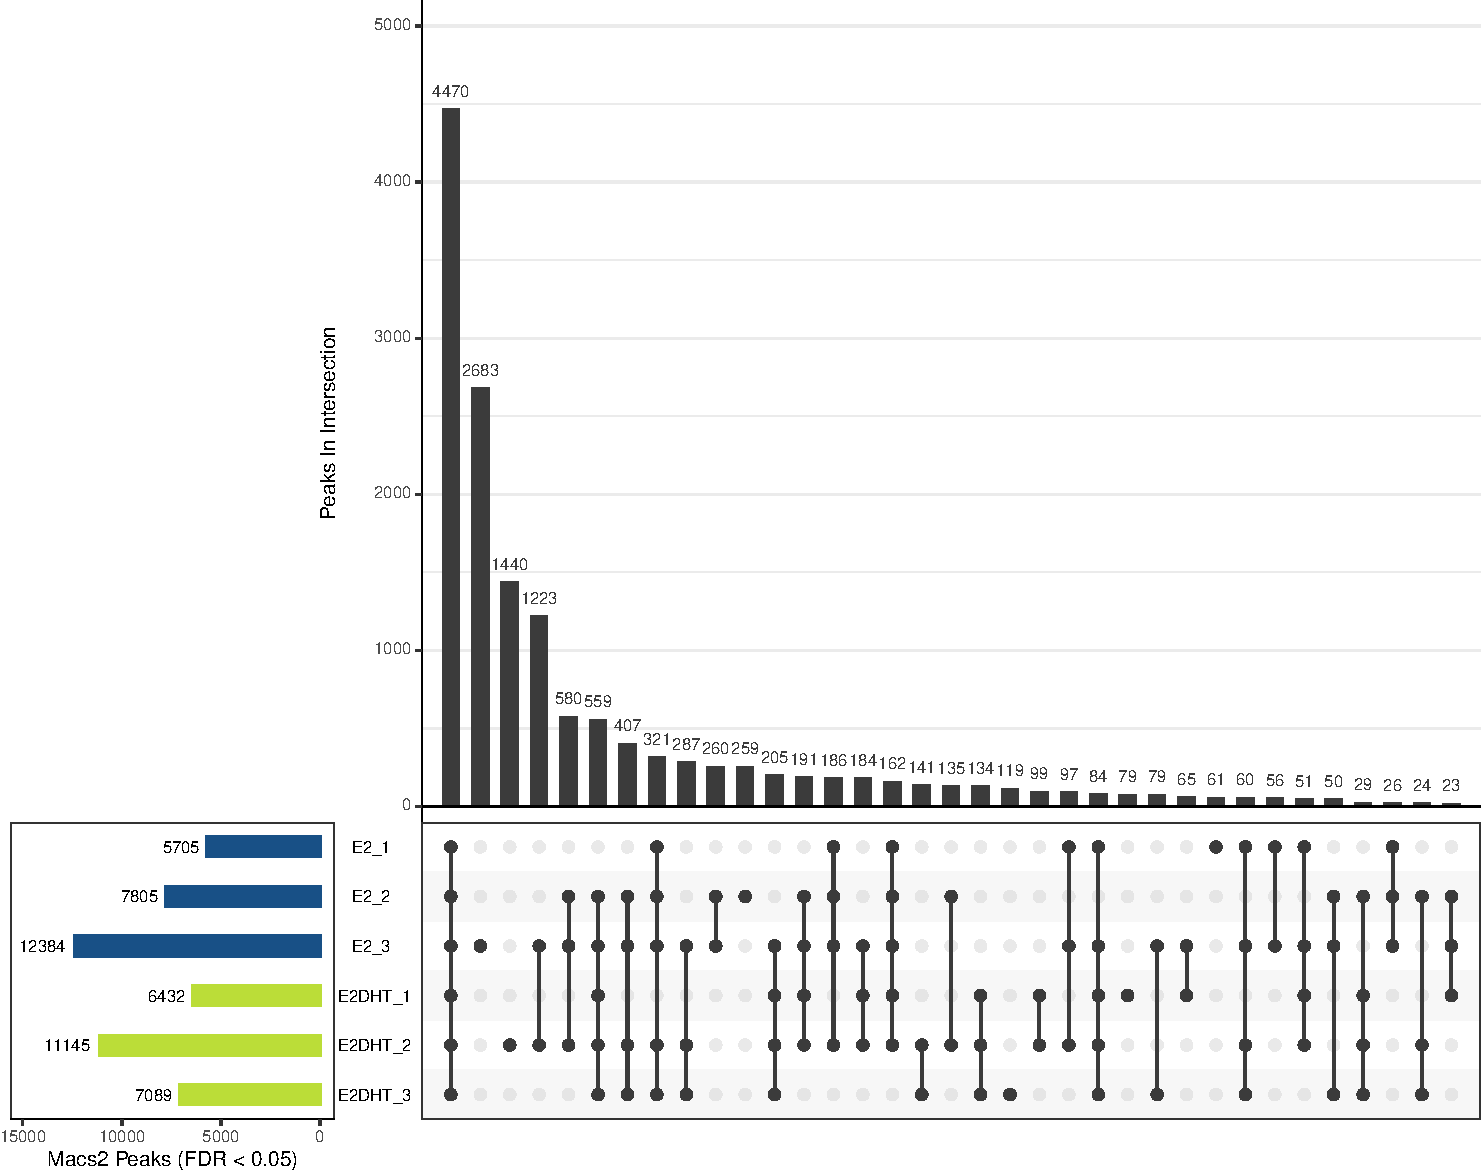
\includegraphics[width=0.35\linewidth]{all-reps-upset-1}
        	\hfill
        	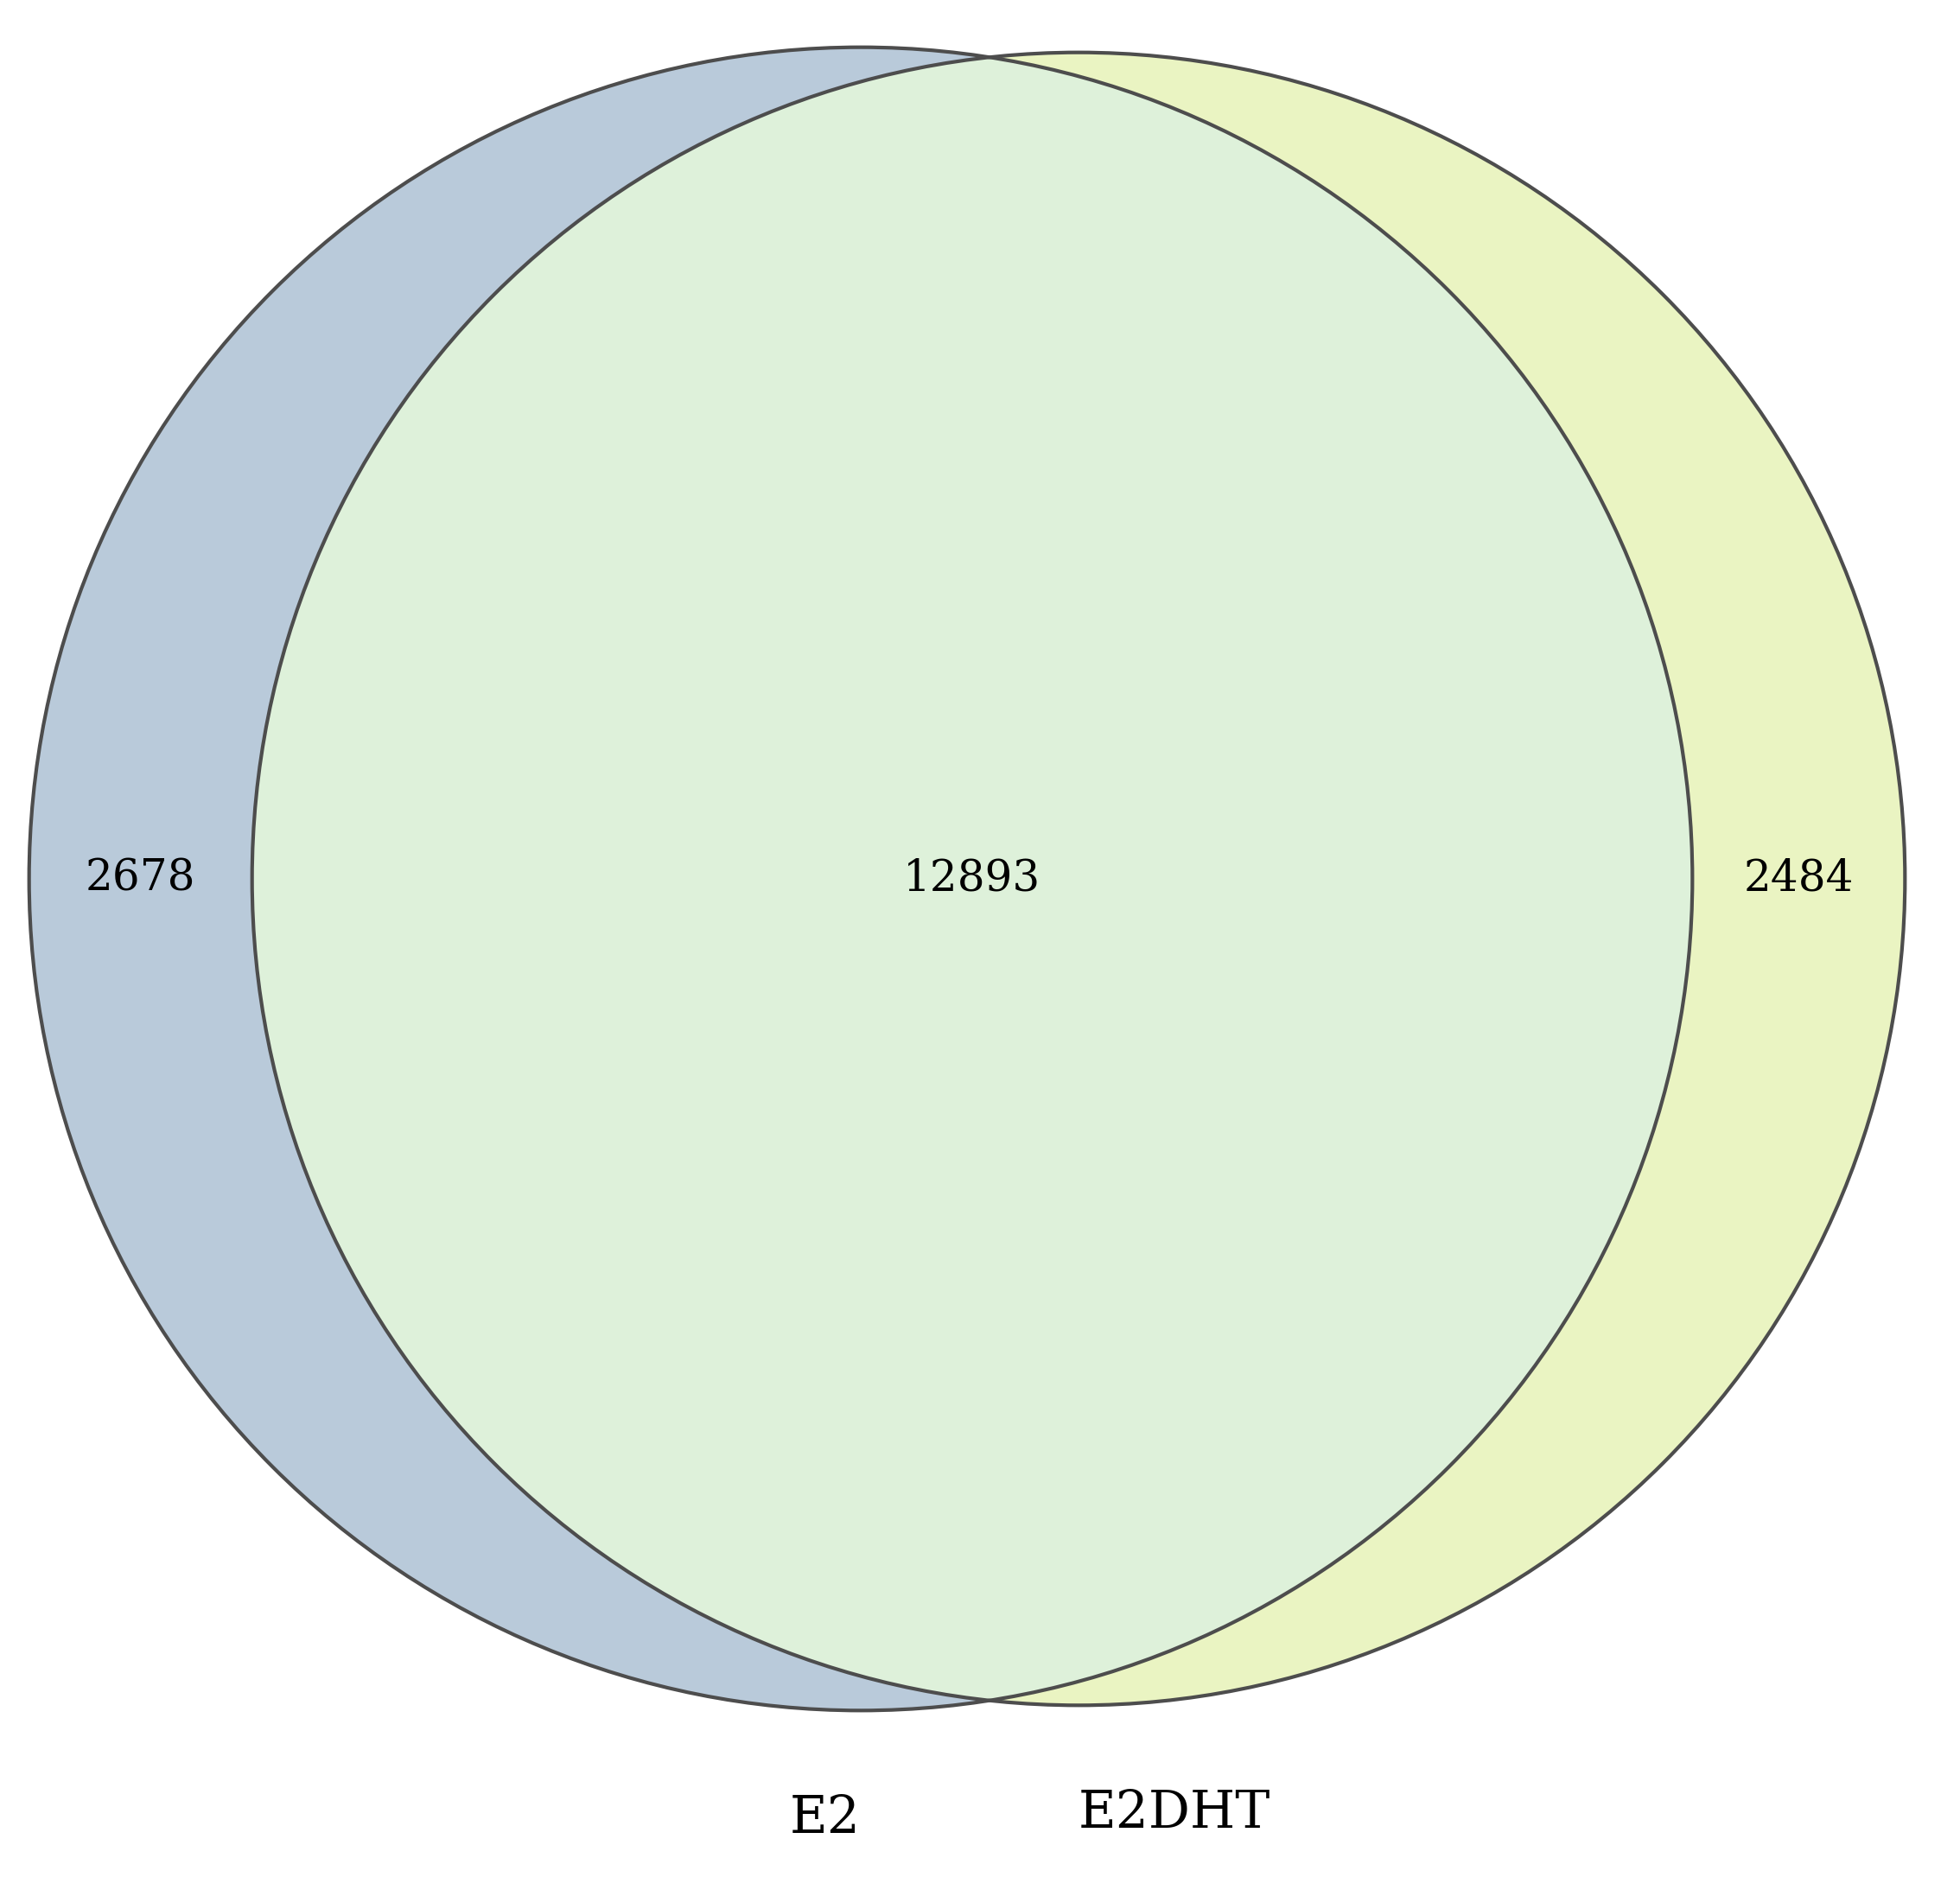
\includegraphics[width=0.25\linewidth]{ER_common_peaks}
        	\hfill
        	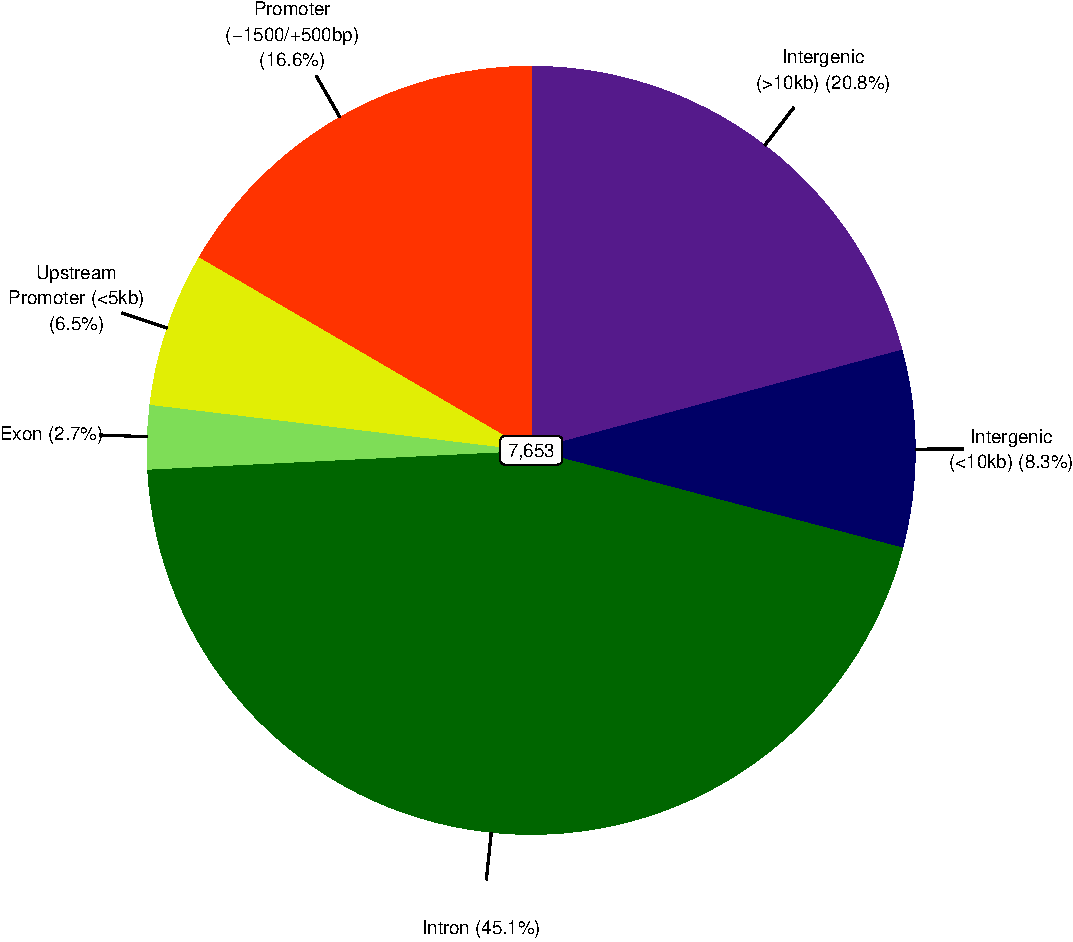
\includegraphics[width=0.3\linewidth]{plot-region-overlap-1}
        \end{tikzfigure}
    	
    }
    \block{Differential Binding}{
    	Differential Binding analysis is performed using sliding windows\cite{csaw} then converting retained windows to \texttt{logCPM} values and normalising using Smooth-Quantile Normalisation\cite{sqn} (Figure \ref{fig:logCPM}) and assessing differential binding using \texttt{limma-trend}\cite{voom}.
    	A range-based $H_0$\cite{treat} is used with the default set to a change in binding $<20$\% being not of interest.
    	Representative windows for a combined region are chosen based on the window with maximal signal.
    	Before final p-value adjustment, weighted p-values are calculated using Independent Hypothesis Weighting using either 1) Genomic Region, 2) External Features or 3) Detection of additional targets (Figure \ref{fig:ihw}).
    	The p-value adjustment method and significance threshold are able to be specified by the user in an experiment-wide manner.
    	Standard sets of result tables are produced as interactive tables, along with MA-plots, profile heatmaps and genomic distributions etc.\\
    	
		\begin{minipage}{0.5\linewidth}
			\centering
	    	\begin{tikzfigure}[Example showing logCPM values for AR before and after Smooth Quantile Normalisation. AR is primarily cytoplasmic under E2 then shifts to be nuclear under E2+DHT\label{fig:logCPM}]
	        	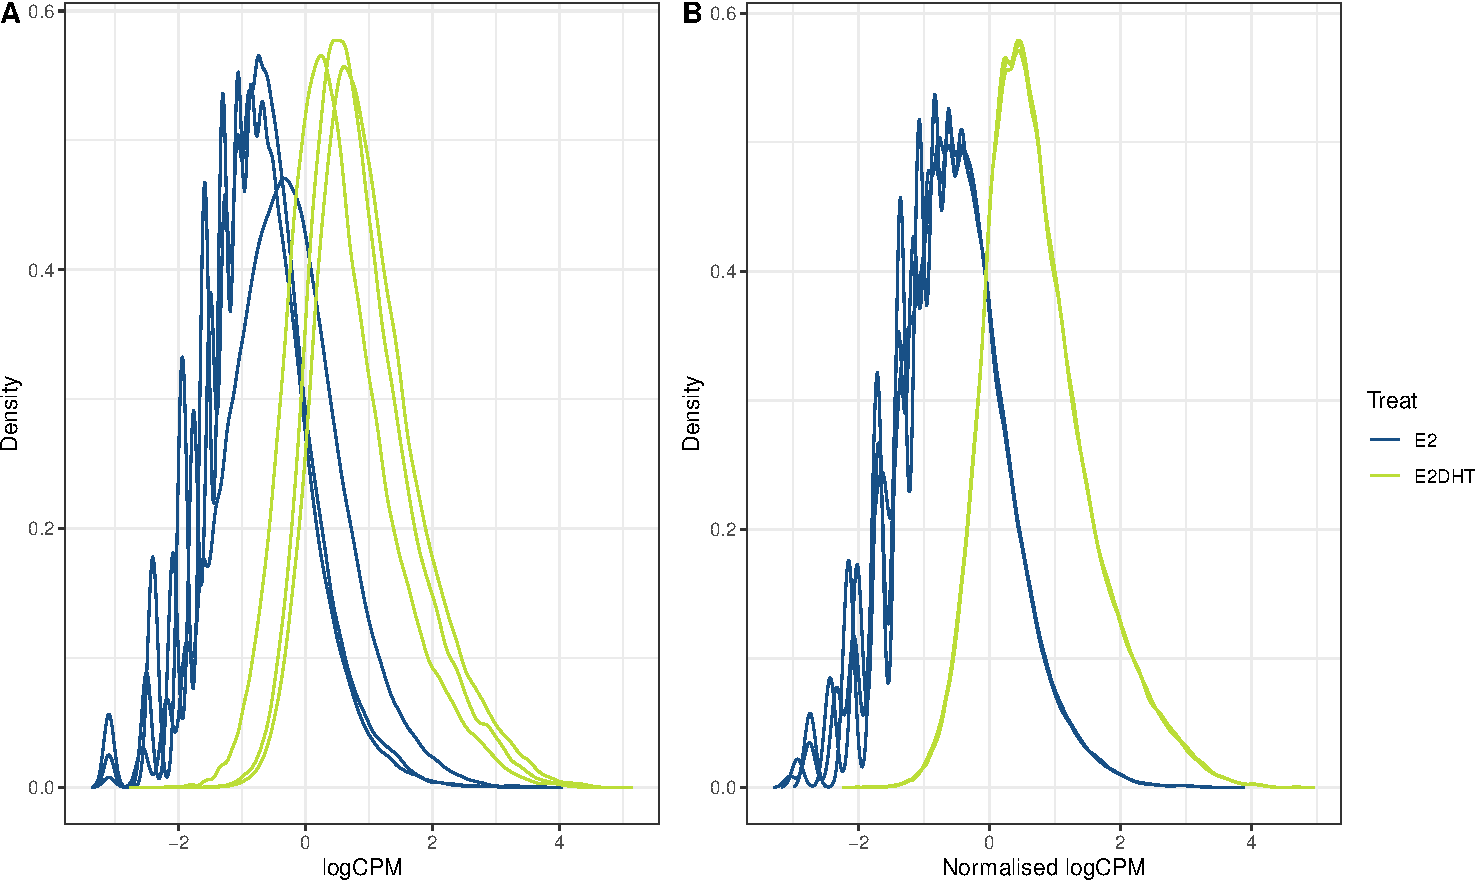
\includegraphics[width=0.9\linewidth]{plot-logcpm-densities-1}
	        \end{tikzfigure}		
		\end{minipage}
  		\begin{minipage}{0.5\linewidth}
  			\centering
           \begin{tikzfigure}[Partitioned p-values for the GATA3 binding response to DHT based on co-detection of the additional ChIP targets AR and ER.\label{fig:ihw}]
	        	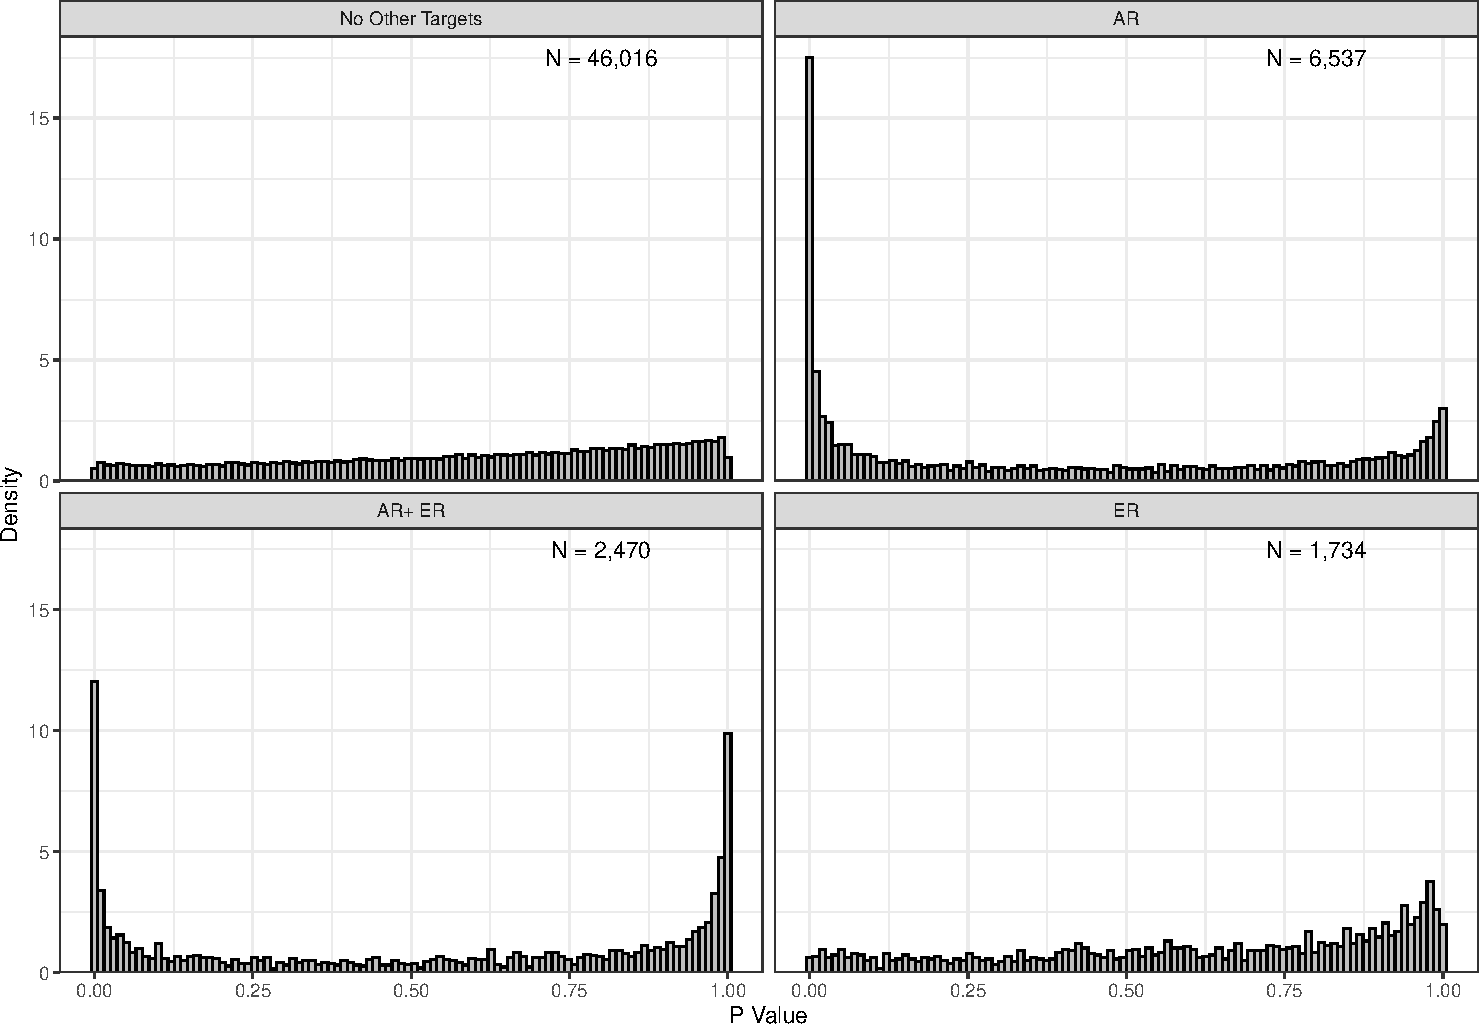
\includegraphics[width=0.8\linewidth]{plot-ihw-pvals-1}
    	    \end{tikzfigure}	
    	\end{minipage}
    	
    	\vspace{8mm}
    	All regions are mapped to genes using \texttt{extraChIPs::mapByFeature()} which maps sites to genes based on which feature type it overlaps.
    	\textbf{Any long-range interactions provided are used to provide more comprehensive mappings} at this point.
    	If \textbf{RNA-Seq} results are provided an additional step is performed assessing the relationship between differentially expressed (DE) genes and any binding sites, directly identifying candidate sites with an observed response at the RNA level.
    	Pathway enrichment analysis is also performed with and without RNA-Seq data.

    	
    }

    \column{0.32}
    \block{Pairwise Comparisons}{
		Given prior rigour in statistical testing, comparison across pairs of factors becomes more of a \textit{site classification problem}.
		When a site is found to be responsive for one transcription factor a lower p-value threshold is applied to the second factor in any overlapping sites, ensuring \textbf{unchanged sites are classified more accurately} as these are important in a pairwise analysis.
		Each site is classified across both ChIP targets as \textit{Up, Down, Unchanged or Undetected} yielding a set of pairwise classifications.
		Comparisons of changed binding (Figure \ref{fig:pairwise-logfc}) are generated across all sites, and separated by annotated region or external feature.
		Profile heatmaps are also created (Figure \ref{fig:heatmap-ar-er}) and enrichment testing is performed on each set of regions.
		Example sites for each set of regions are also plotted by default using \texttt{extraChIPs::plotHFGC()} (Figure \ref{fig:zbtb16}).
		If RNA-Seq data is provided, an analysis of DE genes by pairwise changes in ChIP target binding is also performed (Figure \ref{fig:volcano})
		
		
		\begin{minipage}{0.5\linewidth}
			\centering
           \begin{tikzfigure}[Pairwise logFC values for AR and ER broken down by externally provided H3K27ac-defined features.\label{fig:pairwise-logfc}]
	        	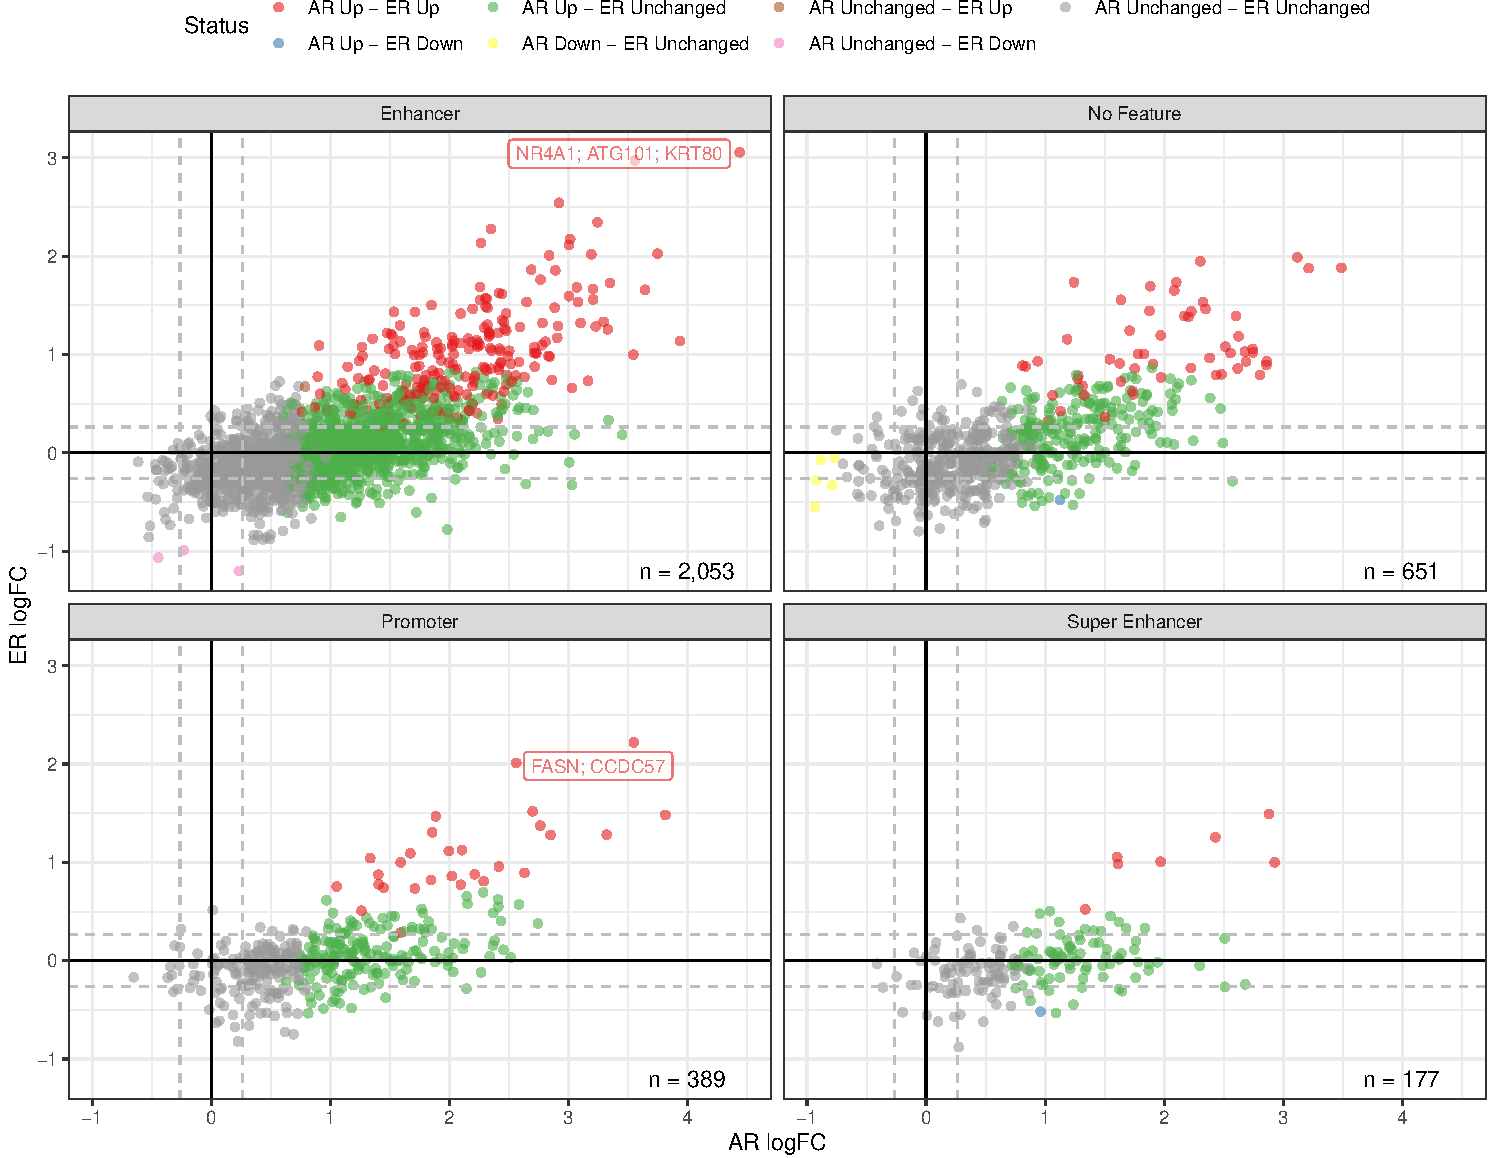
\includegraphics[width=0.9\linewidth]{plot-dbwin-by-feature-1}
    	    \end{tikzfigure}		
		\end{minipage}
  		\begin{minipage}{0.5\linewidth}
  			\centering
	    	\begin{tikzfigure}[Profile heatmap for sites showing increased binding for both AR and ER.\label{fig:heatmap-ar-er}]
	        	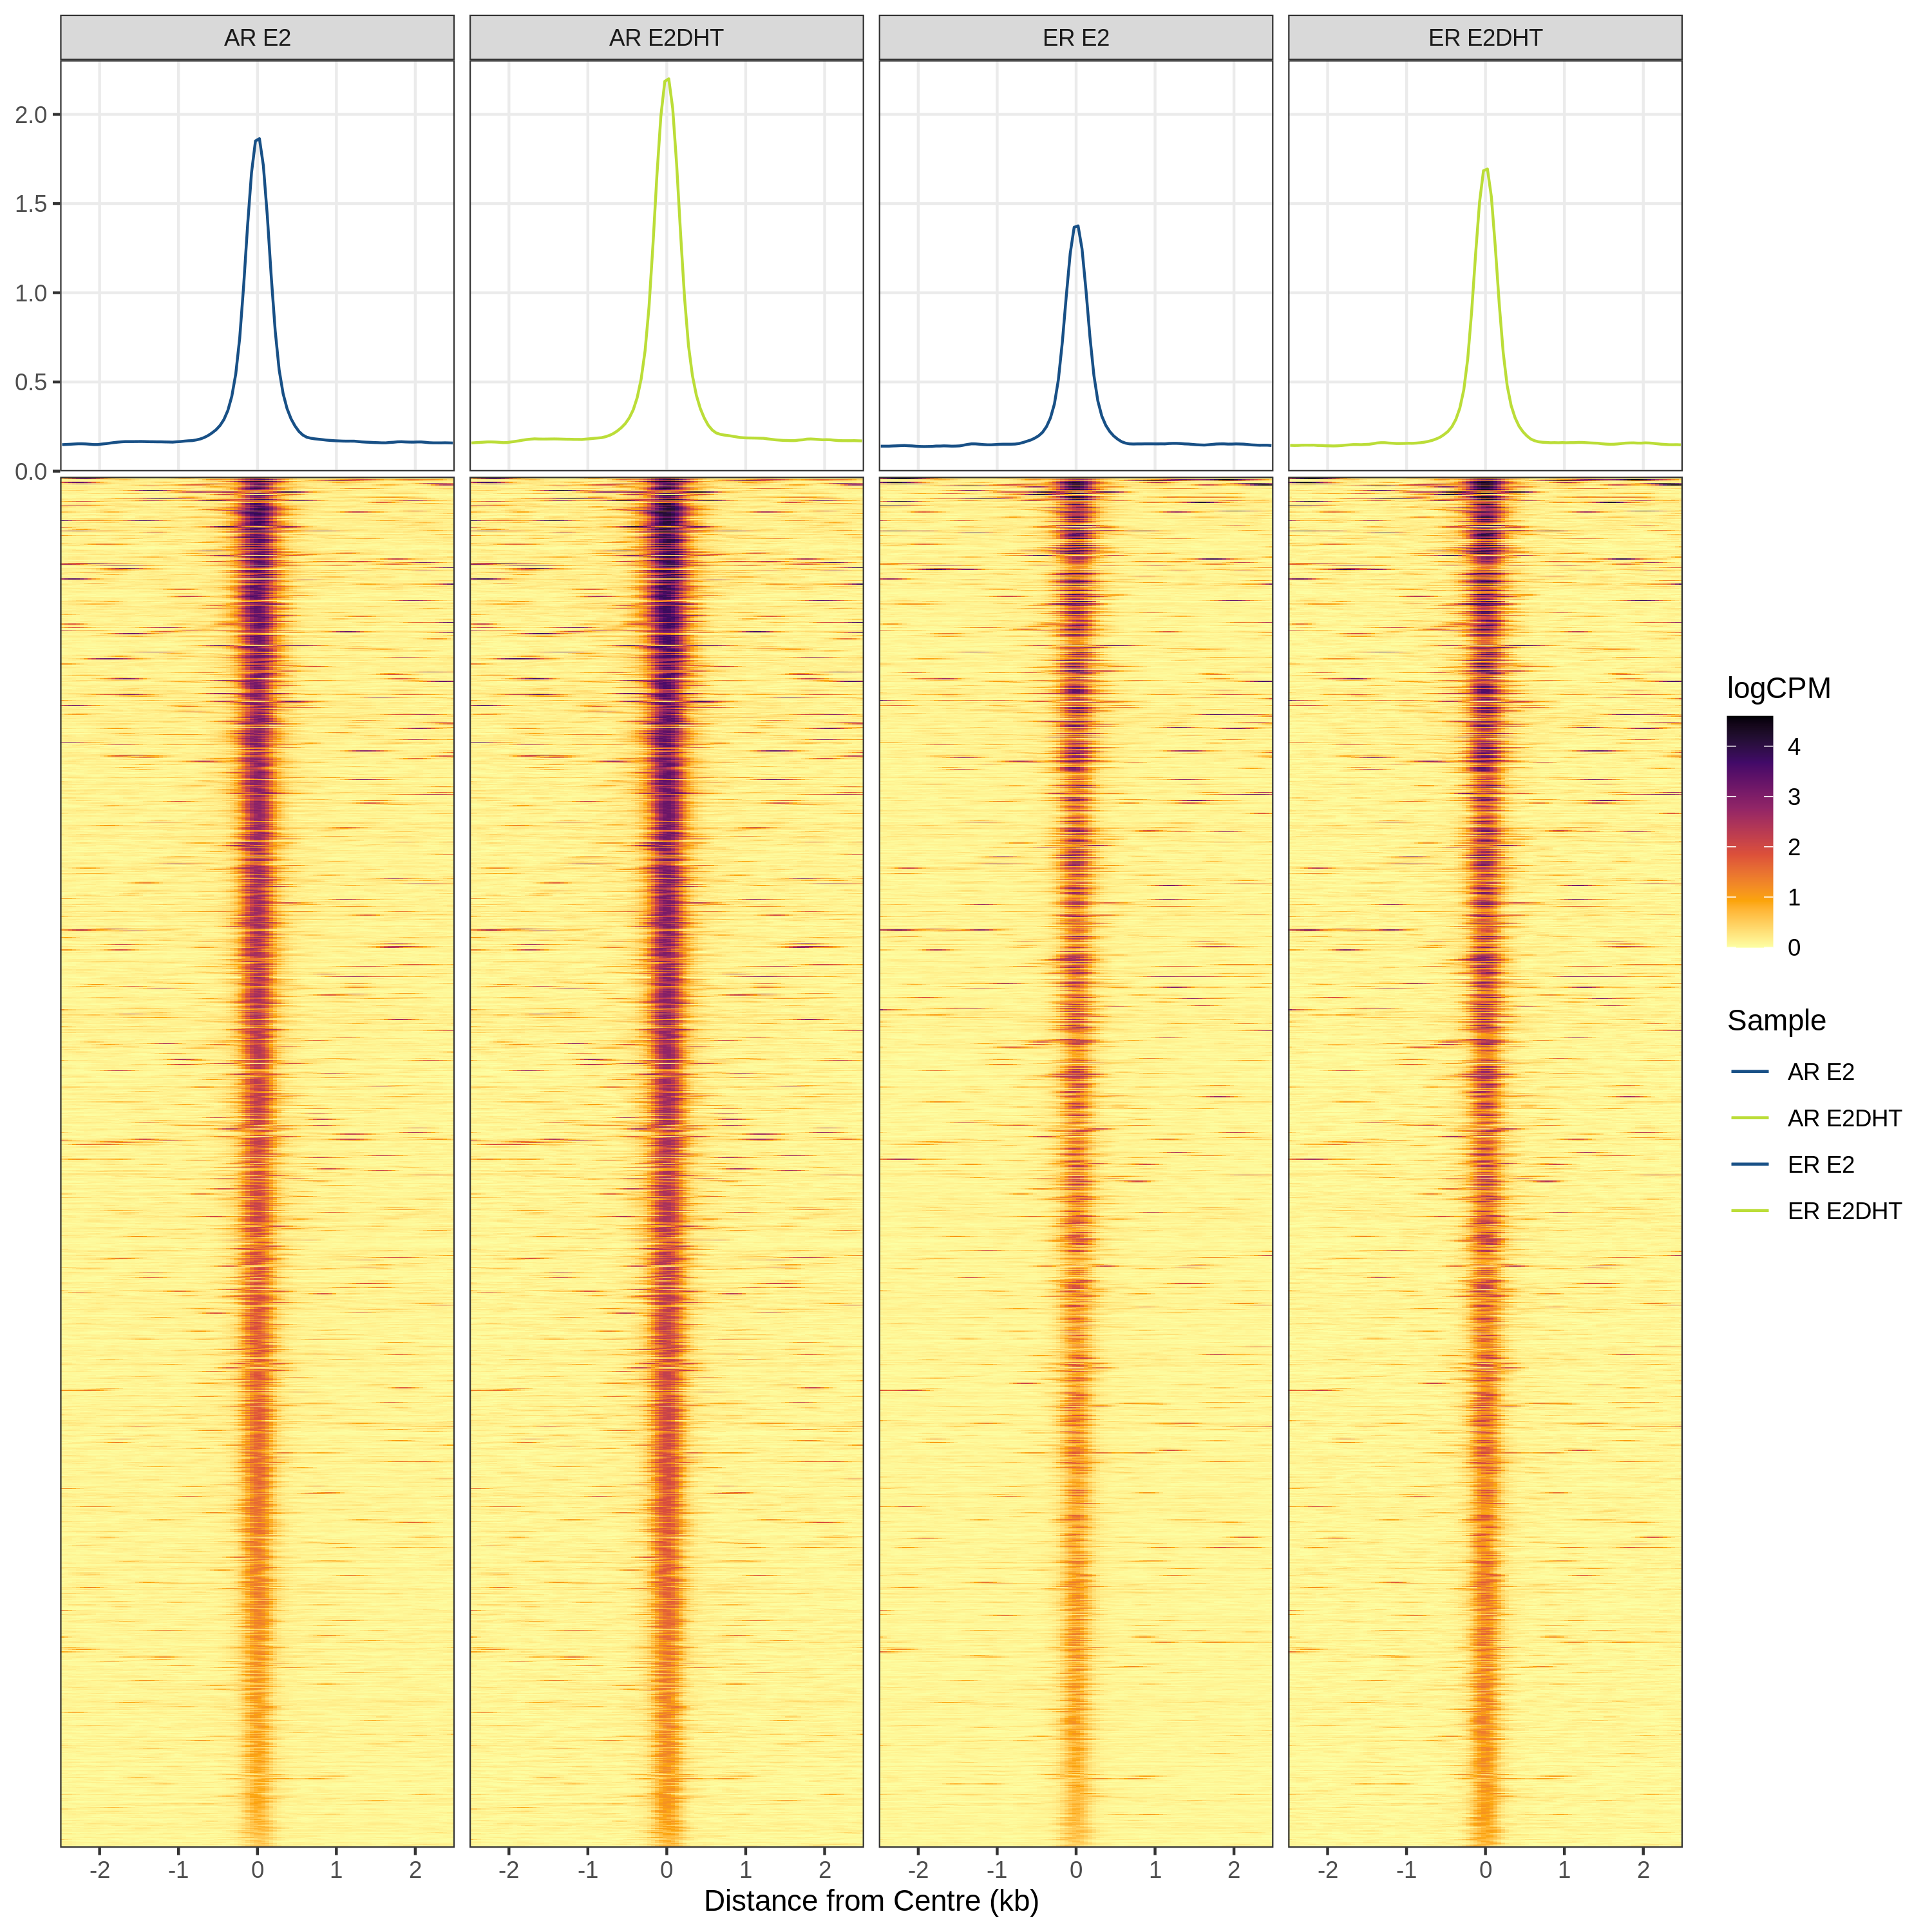
\includegraphics[width=0.7\linewidth]{AR_Up_ER_Up_profile_heatmap}
	        \end{tikzfigure}
    	\end{minipage}\\[1cm]
    	
		\begin{minipage}{0.5\linewidth}
			\centering
           \begin{tikzfigure}[Binding site for \textit{ZBTB16} showing an increase in both AR and ER along with an increase in H3K27ac\label{fig:zbtb16}]
	        	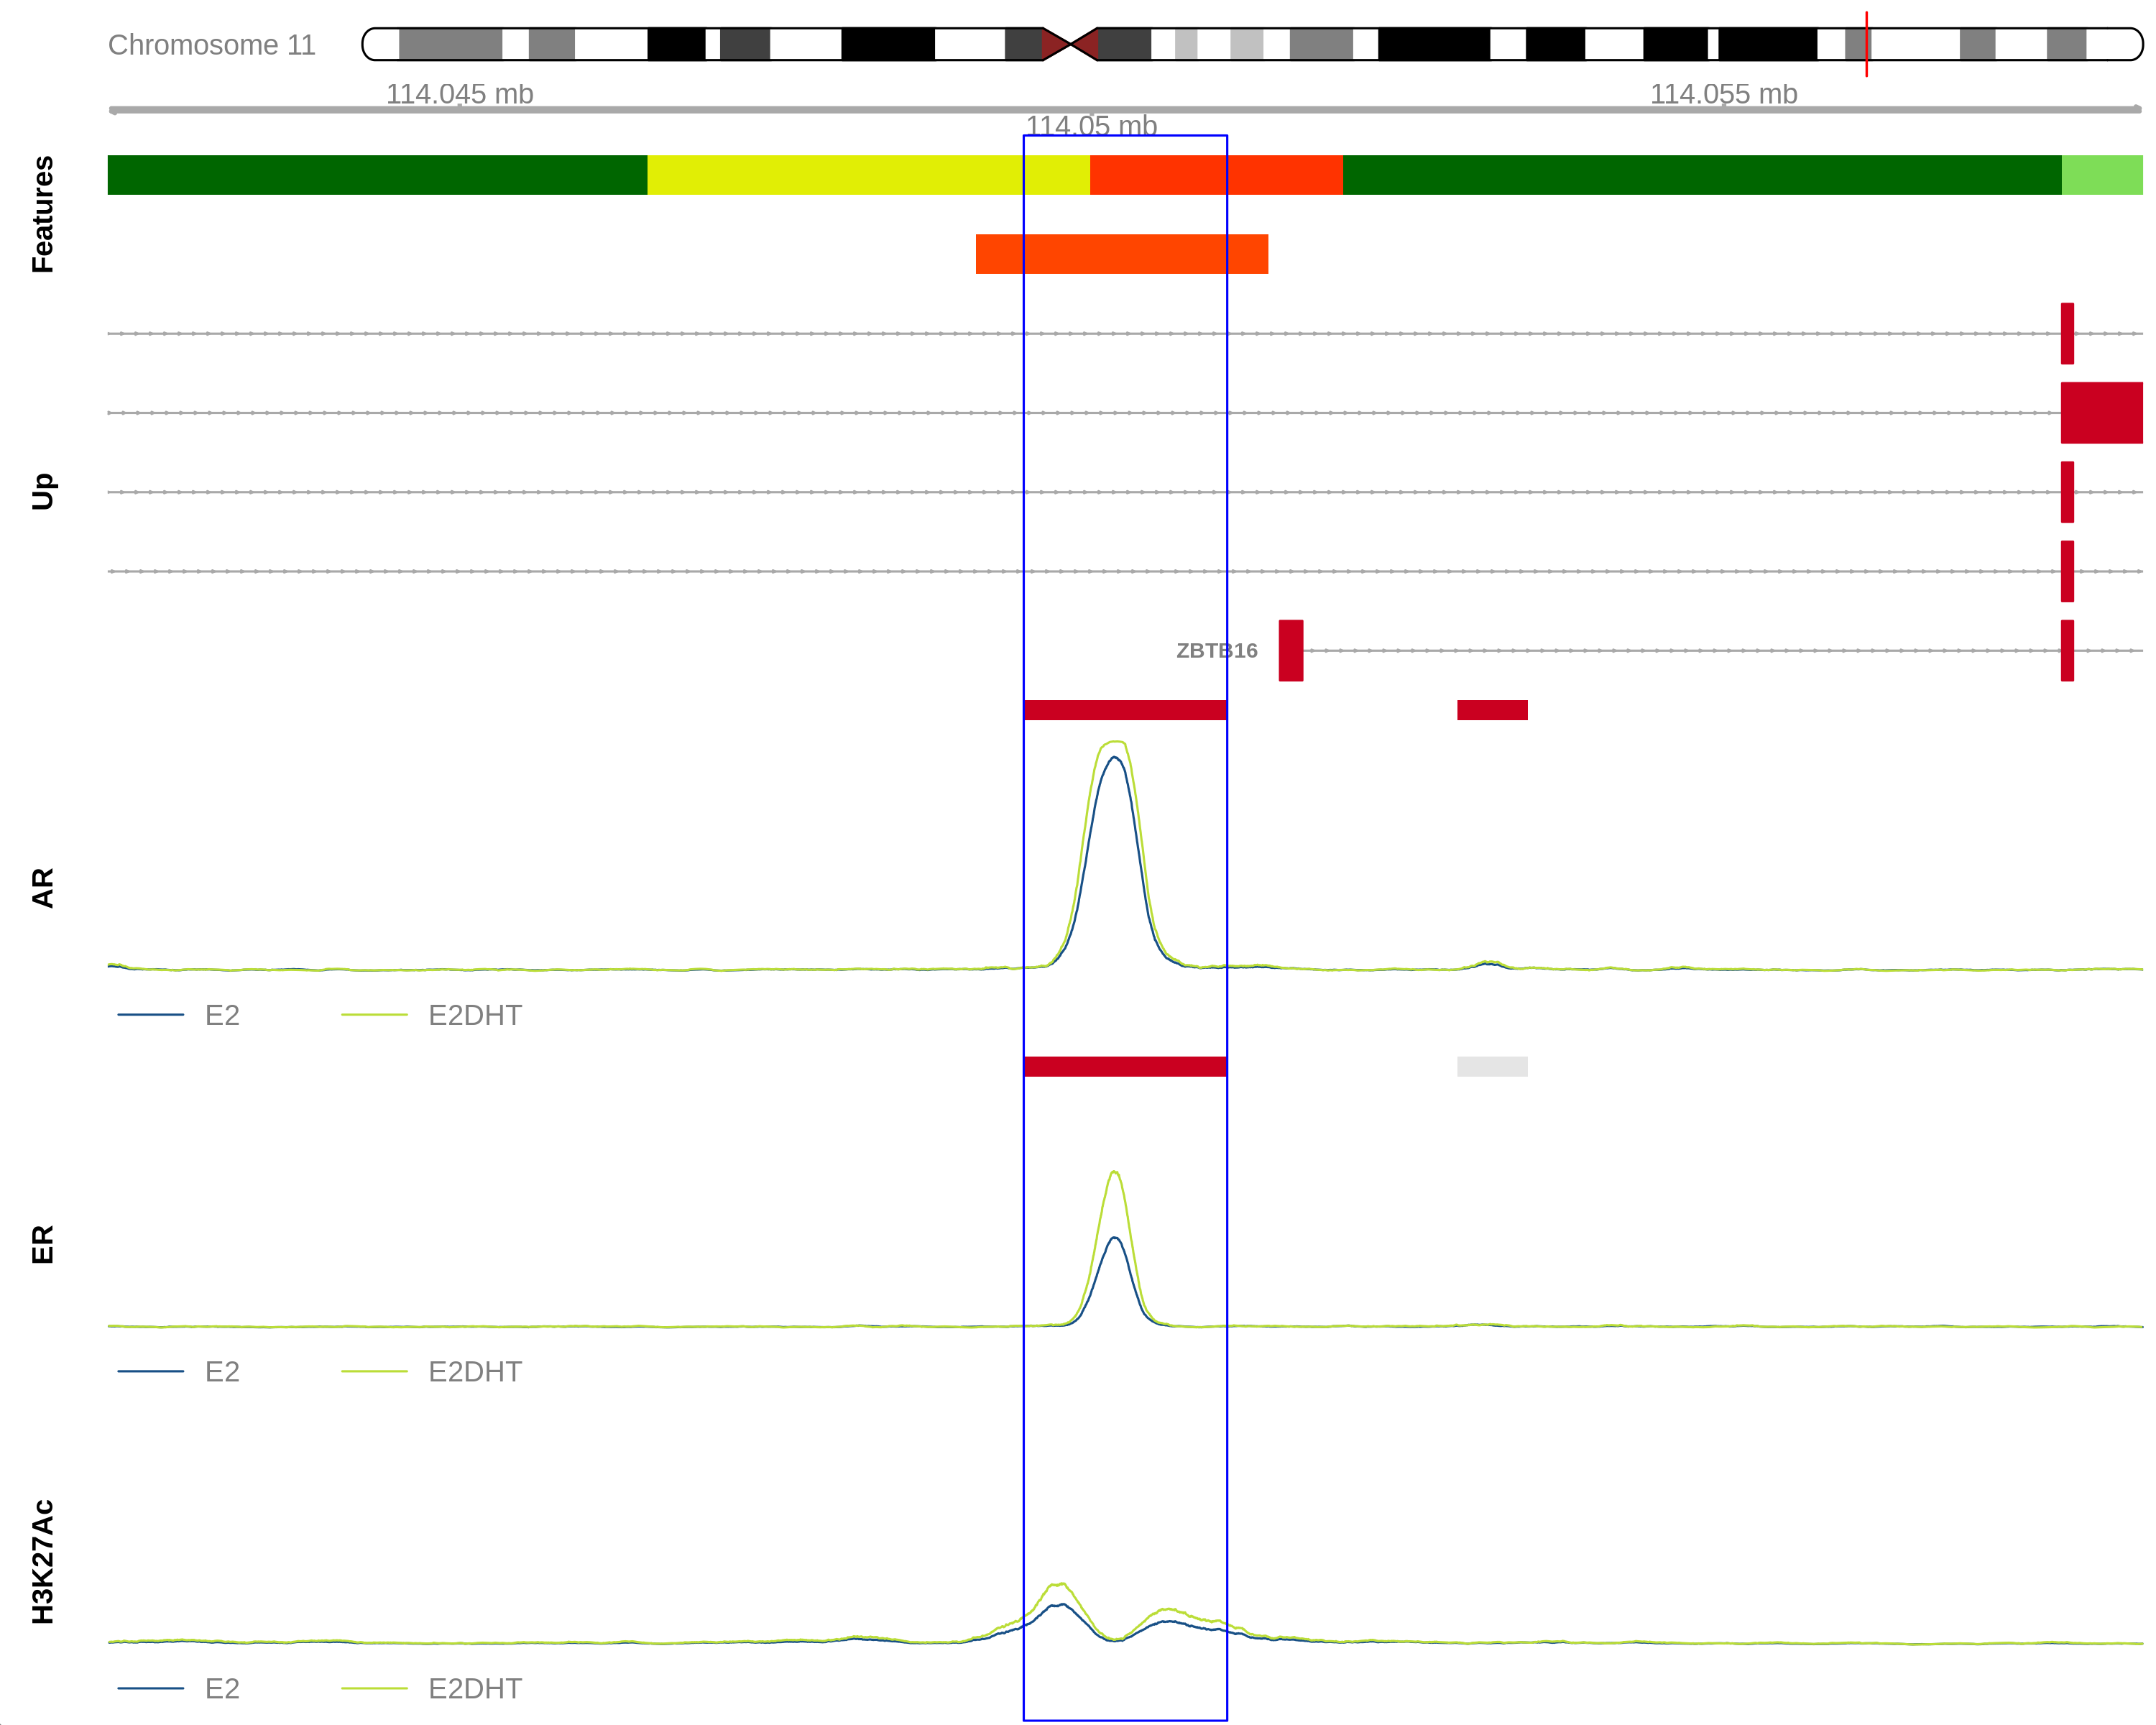
\includegraphics[width=0.8\linewidth]{AR_Up_ER_Up_AveExpr}
    	    \end{tikzfigure}		
		\end{minipage}
  		\begin{minipage}{0.5\linewidth}
  			\centering
           \begin{tikzfigure}[DE Genes by AR and ER binding patterns. Here, the top row would be the most informative.\label{fig:volcano}]
	        	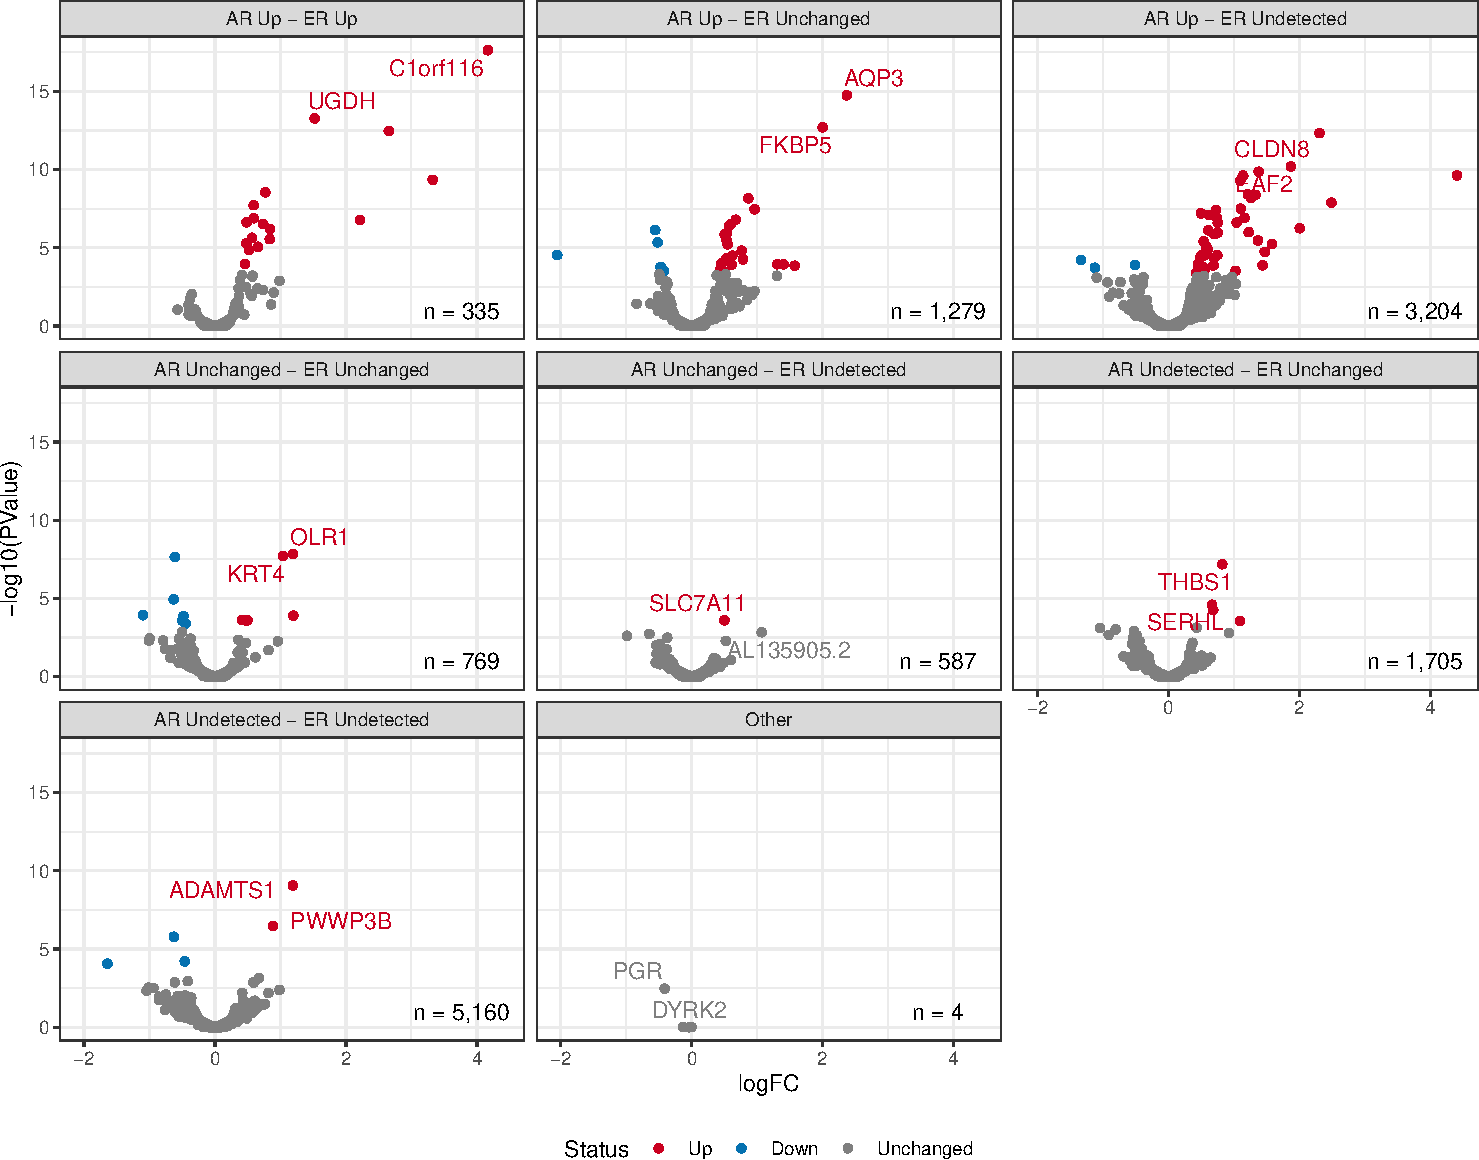
\includegraphics[width=0.85\linewidth]{plot-volcano-1}
    	    \end{tikzfigure}	
    	\end{minipage}

    }
    
    
    \block{References}{
        \vspace{-1em}
        \begin{footnotesize}
        \printbibliography[heading=none]
        \end{footnotesize}
    }
\end{columns}
\end{document}